\documentclass[tikz,border=5pt]{standalone}
\usepackage{luatexja}
\usepackage[hiragino-pron]{luatexja-preset}
\usepackage{amsmath,amssymb}
\usetikzlibrary{arrows.meta,patterns}

\begin{document}
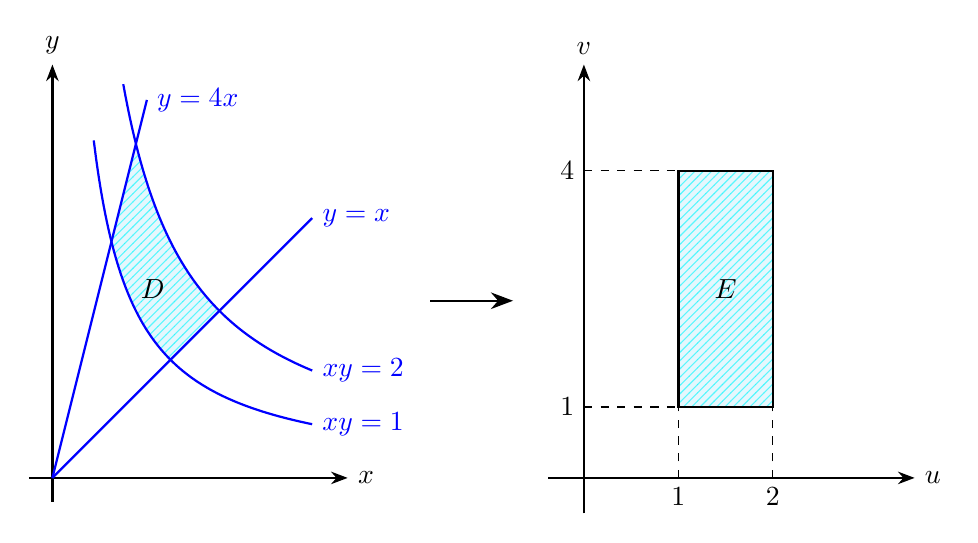
\begin{tikzpicture}[scale=1.5]

% D region (xy-plane, left)
\begin{scope}
  % Axes
  \draw[-{Stealth[length=6pt]}, thick] (-0.2,0) -- (2.5,0) node[right] {$x$};
  \draw[-{Stealth[length=6pt]}, thick] (0,-0.2) -- (0,3.5) node[above] {$y$};

  % Fill region D
  \fill[pattern=north east lines, pattern color=cyan, opacity=0.6]
    plot[domain=1:1.414, samples=2] (\x, \x) --
    plot[domain=1.414:0.707, samples=60, smooth] (\x, {2/\x}) --
    plot[domain=0.707:0.5, samples=2] (\x, {4*\x}) --
    plot[domain=0.5:1, samples=60, smooth] (\x, {1/\x}) -- cycle;
  \fill[cyan, opacity=0.1]
    plot[domain=1:1.414, samples=2] (\x, \x) --
    plot[domain=1.414:0.707, samples=60, smooth] (\x, {2/\x}) --
    plot[domain=0.707:0.5, samples=2] (\x, {4*\x}) --
    plot[domain=0.5:1, samples=60, smooth] (\x, {1/\x}) -- cycle;

  % Lines y=x and y=4x
  \draw[thick, blue, domain=0:2.2, samples=2] plot (\x, \x) node[right] {$y = x$};
  \draw[thick, blue, domain=0:0.8, samples=2] plot (\x, {4*\x}) node[right] {$y = 4x$};

  % Hyperbolas xy=1 and xy=2
  \draw[thick, blue, domain=0.35:2.2, samples=80, smooth] plot (\x, {1/\x}) node[right] {$xy = 1$};
  \draw[thick, blue, domain=0.6:2.2, samples=80, smooth] plot (\x, {2/\x}) node[right] {$xy = 2$};

  % Label
  \node at (0.85,1.6) {$D$};
\end{scope}

% Arrow
\draw[-{Stealth[length=8pt]}, thick] (3.2,1.5) -- (3.9,1.5);

% E region (uv-plane, right)
\begin{scope}[shift={(4.5,0)}]
  % Axes
  \draw[-{Stealth[length=6pt]}, thick] (-0.3,0) -- (2.8,0) node[right] {$u$};
  \draw[-{Stealth[length=6pt]}, thick] (0,-0.3) -- (0,3.5) node[above] {$v$};

  % Rectangle E
  \fill[pattern=north east lines, pattern color=cyan, opacity=0.6]
    (0.8,0.6) rectangle (1.6,2.6);
  \fill[cyan, opacity=0.1]
    (0.8,0.6) rectangle (1.6,2.6);
  \draw[thick] (0.8,0.6) rectangle (1.6,2.6);

  % Dashed guides
  \draw[dashed, thin] (0.8,0) -- (0.8,0.6);
  \draw[dashed, thin] (1.6,0) -- (1.6,0.6);
  \draw[dashed, thin] (0,0.6) -- (0.8,0.6);
  \draw[dashed, thin] (0,2.6) -- (0.8,2.6);

  % Labels
  \node[below] at (0.8,0) {$1$};
  \node[below] at (1.6,0) {$2$};
  \node[left] at (0,0.6) {$1$};
  \node[left] at (0,2.6) {$4$};
  \node at (1.2,1.6) {$E$};
\end{scope}

\end{tikzpicture}
\end{document}
